% TikZ Diagram: Strict zero-data-leakage evaluation protocol timeline
% Style: Minimal publication palette (Grayscale structural + Single Accent for proposed module)
% Rules: Rectangles = Operations/Modules, Rounded = Data/Tensors. Left-to-right flow. Zero line crossing.

\documentclass[tikz,border=10pt]{standalone}
\usetikzlibrary{shapes.geometric, positioning, arrows.meta, chains, backgrounds}

\definecolor{neutralbg}{HTML}{F8FAFC}
\definecolor{neutralstroke}{HTML}{64748B}
\definecolor{neutraltext}{HTML}{0F172A}

\definecolor{accentbg}{HTML}{FEF3C7}
\definecolor{accentstroke}{HTML}{D97706}
\definecolor{accenttext}{HTML}{92400E}

\begin{document}
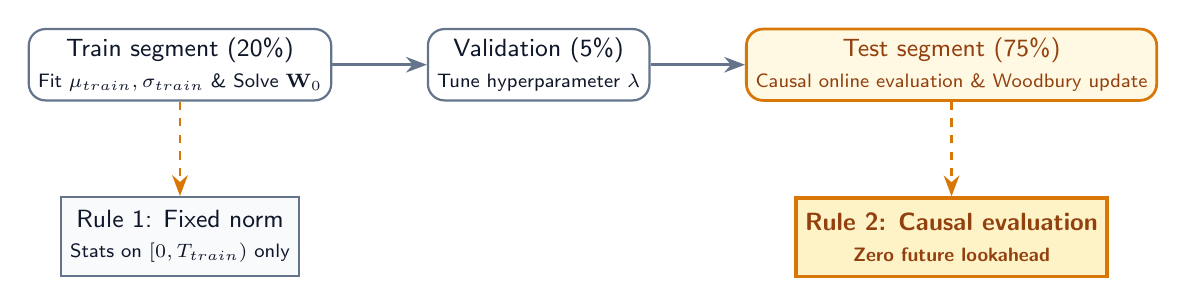
\begin{tikzpicture}[
    font=\sffamily\small,
    node distance=1.0cm and 1.2cm,
    operation/.style={rectangle, draw=neutralstroke, fill=neutralbg, text=neutraltext, minimum height=1.0cm, minimum width=2.2cm, align=center, line width=0.8pt},
    proposed_op/.style={rectangle, draw=accentstroke, fill=accentbg, text=accenttext, minimum height=1.0cm, minimum width=2.4cm, align=center, line width=1.2pt, font=\sffamily\bfseries\small},
    tensor/.style={rounded corners=6pt, draw=neutralstroke, fill=white, text=neutraltext, minimum height=0.9cm, minimum width=2.0cm, align=center, line width=0.8pt},
    proposed_tensor/.style={rounded corners=6pt, draw=accentstroke, fill=accentbg!50, text=accenttext, minimum height=0.9cm, minimum width=2.2cm, align=center, line width=1.0pt},
    arrow/.style={-{Stealth[scale=1.0]}, line width=1.0pt, draw=neutralstroke},
    aux_arrow/.style={-{Stealth[scale=1.0]}, line width=1.0pt, draw=accentstroke, dashed}
]

    % Segments
    \node[tensor] (train) {Train segment (20\%)\\{\scriptsize Fit $\mu_{\text{train}}, \sigma_{\text{train}}$ \& Solve $\mathbf{W}_0$}};
    \node[tensor, right=of train] (val) {Validation (5\%)\\{\scriptsize Tune hyperparameter $\lambda$}};
    \node[proposed_tensor, right=of val] (test) {Test segment (75\%)\\{\scriptsize Causal online evaluation \& Woodbury update}};

    % Timeline arrow
    \draw[arrow] (train) -- (val);
    \draw[arrow] (val) -- (test);

    % Causal boundary rules
    \node[operation, below=1.2cm of train] (r1) {Rule 1: Fixed norm\\{\scriptsize Stats on $[0, T_{\text{train}})$ only}};
    \node[proposed_op, below=1.2cm of test] (r2) {Rule 2: Causal evaluation\\{\scriptsize Zero future lookahead}};

    \draw[aux_arrow] (train) -- (r1);
    \draw[aux_arrow] (test) -- (r2);

\end{tikzpicture}
\end{document}
